% LinkMate - Phase 2 Prototype Progress Report (CECS 451, CSULB Fall 2026)
% Limit: max. 2 pages. Must include the GitHub repository URL.
% Writing rule: no colons in running text.
% Compile: tectonic progress_report.tex   (or latexmk -pdf, or upload to Overleaf)

\documentclass[10pt,letterpaper]{article}

\usepackage[margin=1.7cm]{geometry}
\usepackage[T1]{fontenc}
\usepackage[utf8]{inputenc}
\usepackage{lmodern}
\usepackage{microtype}
\usepackage{graphicx}
\usepackage{booktabs}
\usepackage{tabularx}
\usepackage{enumitem}
\usepackage{xcolor}
\usepackage{titlesec}
\usepackage[hidelinks]{hyperref}

\setlist{nosep, leftmargin=*}
\setlength{\parskip}{2pt}
\setlength{\parindent}{0pt}
\titlespacing*{\section}{0pt}{5pt}{1pt}
\titleformat{\section}{\normalsize\bfseries}{\thesection.}{0.4em}{}
\graphicspath{{../figures/}}

% Visible marker for what the team still has to confirm. Remove the color before submission.
\newcommand{\confirm}[1]{\textcolor{red}{#1}}

\newcommand{\repourl}{\confirm{[GitHub URL]}}

\begin{document}

\begin{center}
  {\Large\bfseries LinkMate}\\[1pt]
  CECS 451 Term Project, Team 10 \quad|\quad Phase 2: Prototype Progress Report\\[1pt]
  Antoine Courant, Felix Baechle, Vishal Bahatyani, Mika Brueggemann\\[1pt]
  Repository: \repourl
\end{center}

\section{Project Objective and Current Scope}
LinkMate helps individuals use the network they already have. It turns free-text notes about people into reviewed contact profiles and answers a need in natural language with ranked contacts, a reason and the source notes, or with ``no suitable contact''. Everything runs locally, because the notes hold third-party data. The scope is unchanged since Phase 1. The prototype is a text-only MVP for about 50 contacts. Photo and voice input and imports remain planned.

\section{Completed Features}
\begin{itemize}
  \item \textbf{Capture.} A note or pasted email becomes a proposed profile. The user corrects it and confirms it as a new contact or as an update to a matched contact. A warning appears for values not found in the note and for instruction-like text.
  \item \textbf{Ask.} A need returns up to three contacts with reason, source notes and a strong or weak match label. Keyword, dense and hybrid search are selectable.
  \item \textbf{Contacts and status.} View, edit, export as JSON and delete contacts and notes. Model checks, index sync and rebuild.
  \item \textbf{Engineering.} One-command setup with a double-click start on Mac and Windows, 93 unit tests, end-to-end scenarios and an evaluation suite. Tested on macOS only. The Windows and Linux paths and the automatic Ollama installation are written but not yet run.
\end{itemize}
Milestones M1 to M3 are complete, and this report closes M4. \textbf{Planned, not built}: photo and voice input, email and LinkedIn import, a mobile interface, cloud sync.

\section{System Architecture}
\begin{center}
  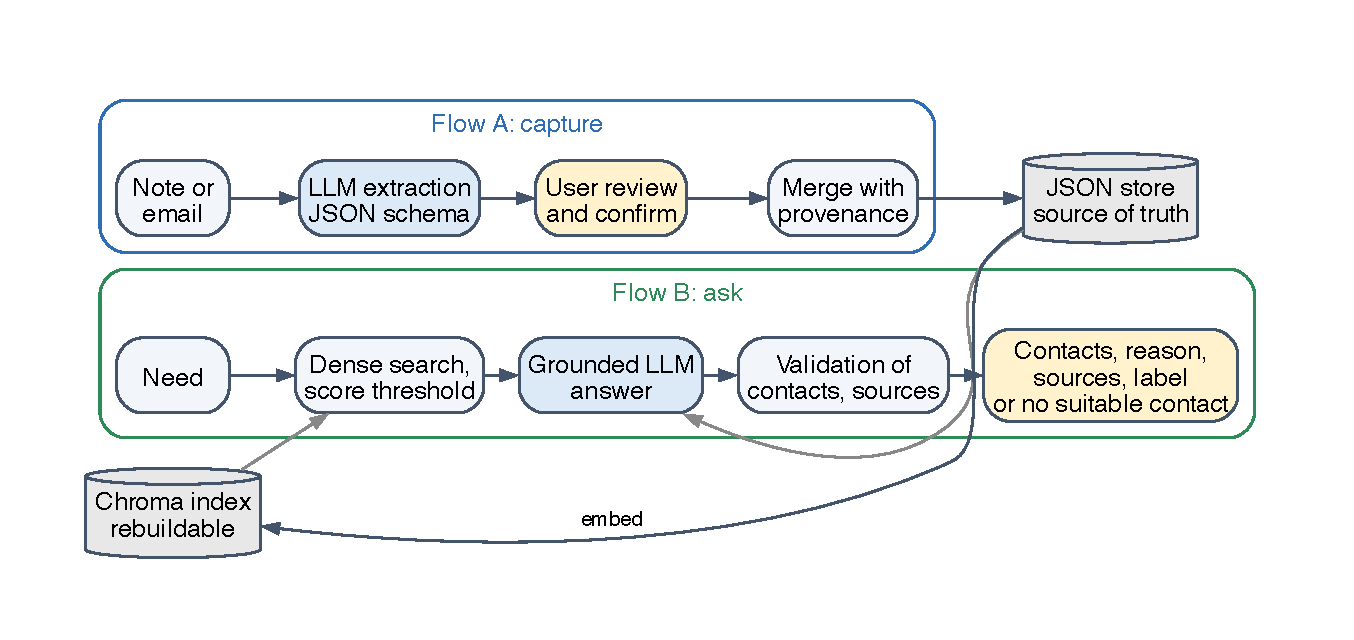
\includegraphics[width=0.74\linewidth]{architecture}
\end{center}
\vspace{-3pt}
Pages call services only, services use a pure core and three infrastructure classes. JSON files are the source of truth, and the Chroma index can be rebuilt from them. The LLM only proposes. It never writes data, never sees real IDs and has no tools. Code resolves its labels and drops any recommendation without a valid source. The full documentation with diagrams, interfaces and 13 design decisions is in \texttt{docs/architecture.md}.

\section{Data and Models}
\textbf{Data.} A synthetic dataset created with LLM support and checked by hand, with 55 fictional contacts and 70 notes, including deliberately vague and long ones. There are 70 labeled questions, 30 for development and 40 held out, each with expected and acceptable contacts. A quarter of the held-out questions have no right answer, most of them with a near miss.

\textbf{Models.} \texttt{qwen3:0.6b} (0.5 GB on disk, about 0.8 GB in memory) for extraction and answers, with temperature 0 and a JSON schema. \texttt{nomic-embed-text} for embeddings. The larger \texttt{qwen3:1.7b} did worse in the same pipeline and was rejected. Both run through the Ollama HTTP API on an 8 GB laptop, with no API keys. Prompts, input and output behavior and limits are in \texttt{docs/llm\_workflow.md}.

\textbf{Own contribution.} Data model, prompts and schemas, review and merge with provenance, chunking, BM25 and rank fusion, threshold and match label, output validation, injection hardening, interface, setup and evaluation.

\textbf{Baseline.} BM25 keyword search, implemented in \texttt{linkmate/core/retrieval.py}.

\section{Preliminary Results}
Held-out questions, measured with \texttt{eval/evaluate.py}. Settings were frozen on the development questions first.

\begin{center}
\small
\begin{tabular}{@{}lccc@{}}
  \toprule
  System & Right contact (of 30) & Correct refusal (of 10) & Recommendations that fit \\
  \midrule
  Keyword baseline, top hit & 20 (67\%) & 0 (0\%) & 21/39 (54\%) \\
  Dense search, top hit & 23 (77\%) & 1 (10\%) & 26/38 (68\%) \\
  LinkMate, all recommendations & 21 (70\%) & 2 (20\%) & 25/35 (71\%) \\
  LinkMate, strong label only & 16 (53\%) & 9 (90\%) & 16/18 (89\%) \\
  \bottomrule
\end{tabular}
\end{center}

Directly worded needs reach 14/14. Paraphrased needs are the hard part, with 7/16 for LinkMate and Recall@3 of 0.75 for dense search against 0.44 for keywords. No recommendation had an invalid source. Extraction on 70 notes gave no invalid output, 70/70 correct names and a fact F1 of 0.69. A question takes 1.2 s at the median.

\textbf{Example.} ``Who could teach me lead climbing?'' after capturing a note about Mara Lindt returns Mara Lindt with a reason and the note as source. The full input-to-output run can be reproduced with the steps in the README.

\section{Known Limitations}
\begin{itemize}
  \item \textbf{Weak refusals.} The small model accepts near misses, and search scores of fitting and unfitting contacts overlap. Showing weak matches with a label is the current mitigation.
  \item \textbf{Reasons can contain invented details}, so source notes are always shown. The code checks sources, not the wording.
  \item \textbf{Synthetic data, no user test yet.} Notes are cleaner than real ones, and the confidence intervals are wide at this sample size.
  \item \textbf{Prompt injection.} An email telling any AI to recommend its author influenced two answers. Such sentences are now removed by a keyword rule, which new wording can get past, and attacks can still reach the proposed profile. The user review stays mandatory.
\end{itemize}

\section{Remaining Tasks}
\begin{itemize}
  \item User pilot with the prepared protocol for time, success and willingness to pay (\texttt{docs/phase3/user\_pilot.md}).
  \item Run the setup on Windows and Linux.
  \item Pitch video with prototype demo and Combined Final Report, due December 11.
\end{itemize}

\section{Team Responsibilities}
\small
\begin{tabularx}{\linewidth}{@{}lX@{}}
  \toprule
  Member & Current responsibility \\
  \midrule
  Antoine Courant & \confirm{Business case, market evidence, pitch structure} \\
  Felix Baechle & \confirm{Prototype integration, evaluation, technical documentation} \\
  Vishal Bahatyani & \confirm{Repository, AI plan and risks, LLM workflow, user pilot} \\
  Mika Brueggemann & \confirm{Dataset, data pipeline, Windows and Linux testing} \\
  \bottomrule
\end{tabularx}

\end{document}
